\documentclass[mf, pdftex]{mgrwms}
\usepackage[utf8]{inputenc}
\usepackage{amsmath}
\newcommand\numberthis{\addtocounter{equation}{1}\tag{\theequation}}
\usepackage{amssymb} 
\usepackage{bbm}
\usepackage{mathtools}
\usepackage{latexsym}
\usepackage{amsthm}
\usepackage{enumerate}
\usepackage{color}
\usepackage[polish]{babel}
\usepackage[OT4]{fontenc}
\usepackage{polski}
\usepackage{graphicx}
\usepackage{float}
\usepackage{placeins}

\graphicspath{{Figs}}
\bibliographystyle{apalike}

\allowdisplaybreaks

\begin{document}

\title{\LARGE Zastosowanie modeli kopułowych do modelowania spreadu aktywów}
\author{Piotr Mikler}
\promotor{dr inż. Jerzy Dzieża}
\nralbumu{409145}
\maketitle
\slowakluczowe{spread, soja, opcje, copuła, vine copula}
\keywords{spread, soybean, option, copula, vine copula}

\newtheorem{thm}{\indent Twierdzenie}[chapter]
\newtheorem{lemma}[thm]{\indent Lemat}
\newtheorem{cor}[thm]{\indent Wniosek}
\newtheorem{obs}[thm]{\indent Obserwacja}
\newtheorem{prop}[thm]{\indent Własność}
\newtheorem{uw}[thm]{\indent Uwaga}
\newtheorem{df}[thm]{Definicja}
\newcommand{\E}{\mathbb{E}}
\newcommand{\R}{\mathbb{R}}
\newcommand{\Pra}{\mathbb{P}}
\newcommand{\1}{\mathbbm{1}}
\newcommand{\Corr}{\text{Cor}}
\newcommand{\Cov}{\text{Cov}}
\newcommand{\Var}{\text{Var}}

\makeatletter
\newcommand*{\defeq}{\mathrel{\rlap{%
                     \raisebox{0.3ex}{$\m@th\cdot$}}%
                     \raisebox{-0.3ex}{$\m@th\cdot$}}%
                     =}
\let\c@table\c@figure
\makeatother


%% --- BODY --- %%
\begin{streszczenie}
	Spready grają dziś ogromną rolę na rynkach finansowych. Służą inwestorom, spekulantom i zarządzającym ryzykiem do oceny potencjalnych zysków z inwestycji, implikowania zmiennych rynkowych, czy kontrolowania ekspozycji na ryzyko. W pracy prezentujemy modele kopułowe jako narzędzia odpowiednie do statystycznej analizy współzależności między komponentami spreadu. 
	
	Literatura bogata jest w przykłady zastosowania dwuwymiarowych kopuł do modelowania dwuwymiarowych spreadów. Te modele, oparte o połączenie analizy szeregów czasowych oraz modelowania reziduów przy pomocy kopuł stały się jednym z klasycznych podejść do problemu wyceny instrumentów pochodnych na spread. Na początku lat 2000 dodatkowo rozwinęła się teoria modeli Vine Copula, pozwalających na elastyczny opis zależności wielowymiarowych. Od tamtego czasu konsekwentnie odnoszą one sukcesy w modelowaniu zjawisk w wielu dziedzinach nauki, od lotnictwa, przez biologię po finanse. Mimo tego, literatura dotycząca aplikacji Vine Copula do modelowania wielowymiarowych spreadów jest zdecydowanie ograniczona. 
	
	Praca poszerza literaturę Vine Copula o aplikację tych modeli do spreadu na 3 aktywa. Prezentujemy niezbędną teorię, oraz pokazujemy w jaki sposób zbudować symulacyjny model dla soybean crush spread, w którym numerycznie wyceniamy europejskie opcje na soybean crush spread. 
\end{streszczenie}

\begin{abstract}
	Nowadays, spreads play a vital role on global financial markets. They serve both investors, speculators and risk managers alike as a measure of potential investment turnover, to imply market variables, or as tools for controlling market risk exposures associated with combinations of risk factors. In this paper, we present copula models as a suitable tool for statistical modelling of dependency between spread components.
	
	The literature is rich with examples of bivariate copulas applied to model bivariate spreads. These models which are a combination of time series analysis and copulas have become one of the classical solutions to the problem of pricing spread derivatives. In early 2000s the copula theory was extended to Vine Copula models, allowing the flexibility of copulas to be used in higher dimensions. Since then they have been successfully applied to model phenomena in a wide range of industries: from aviation to biology to finance. Nevertheless, the literature on modelling spreads in higher dimensions using Vine Copulas is relatively limited.
	
	This paper extends the literature of Vine Copula models by presenting an application to 3-dimensional spread modelling. We present the necessary theory, and show how to build a simulation model for soybean crush spread, as well as how to numerically price European options on that asset.
	
\end{abstract}

\tableofcontents

\begin{wstep}[Wprowadzenie]
	Celem niniejszej pracy jest zbadanie skuteczności modeli \emph{Vine Copula} w zastosowaniu do modelowania spreadu na różnicę cen 3 instrumentów finansowych. Podajemy teorię niezbędną do zdefiniowania tych modeli, omawiamy obecne podejścia do modelowania spreadu i kalibrujemy model \emph{Vine Copula} do danych rzeczywistych dotyczących \emph{soybean crush spreadu}. W tym modelu numerycznie wyceniamy europejskie opcje na spread.\\
	
	W pierwszym rozdziale wprowadzamy istotne dla teorii kopuł obiekty z zakresu probabilistyki i statystyki. Przedstawiamy wielowymiarowe zmienne losowe, z naciskiem na modele ich rozkładów najczęściej stosowane w praktyce, oraz wskazując na ich istotne ograniczenia. Definiujemy również miary współzależności zmiennych losowych, wychodząc ze statystycznego punktu odniesienia.\\
	
	Drugi rozdział stanowi opis dwuwymiarowych modeli kopułowych i ich rozszerzenia do \emph{Vine Copulas}. Definiujemy w nim dwuwymiarowe kopuły, podajemy przykłady i pokazujemy że są rozszerzeniem rozkładów wielowymiarowych z rozdziału pierwszego. Redefiniujemy przy tym również miary współzależności z rodziału pierwszego, tym razem w języku kopuł.\\
	
	W rozdziale trzecim skupiamy się na pojęciu spreadu aktywów, podajemy ich przykłady obecne na rynkach finansowych i wymieniamy podejścia do ich modelowania. Skupiamy się na podejściu kopułowym, łączącym modelowanie szeregów czasowych z wielowymiarowymi kopułami - w szczególności ze strukturami \emph{Vine Copulas}.\\
	
	Ostatni rozdział prezentuje wynik kalibracji modelu do rzeczywistych danych, tj. cen \emph{soybean crush spread}, czyli różnicy między ceną surowca (ziaren soi), a powstających z niej produktów: mączki sojowej i olejku sojowego. Pokazujemy jak w numeryczny sposób można wycenić w tym modelu opcje europejskie, oraz porównujemy wyniki symulacji modelu używającego \emph{Vine Copula}, a najprostszego modelu wielowymiarowej kopuły gaussowskiej.
	
\end{wstep}

\chapter{Wielowymiarowe zmienne losowe}
W klasycznym studium doboru struktury portfela (\cite{Markovitz_MPT}), Markovitz analizuje portfel aktywów. Przedmiotem tej pracy jest opis sposobu, w jaki indywidualne pozycje w portfelu wpływają na jego całościowy zwrot i ryzyko. Współczesna teoria portfela która została zapoczątkowana tą pracą wymaga zamodelowania całego systemu jakim jest zbiór akcji w portfelu. Markovitz pokazuje w swojej pracy istotę współzależności między poszczególnymi aktywami, od której zależy czy ryzyko portfela ulega dywersyfikacji, czy jest amplifikowane. Modelowanie każdego aktywa z osobna jest niewystarczające, ponieważ istota ich wpływu na portfel tkwi w przeważającym stopniu we współzależnościach pomiędzy nimi.\\
Problem wielowymiarowości i poprawnego jej opisu pojawia się nie tylko w finansach, ale w prawie każdej dziedzinie gdzie do realnych problemów aplikuje się modelowanie matematyczne. Zanim wprowadzimy więc pojęcie kopuły, które posłuży nam do analizy wielowymiarowych zależności, w tym rozdziale skupimy się na $d$-wymiarowych wektorach losowych $\mathbf{X} = [X_1, X_2, \dots, X_d]$ i przypomnimy elementy rachunku prawdopodobieństwa i statystyki istotnych z punktu widzenia teorii kopuł.\\

\section{Zmienne losowe}
\label{sec:rozklady_laczne}
Rozpatrywać będziemy przestrzeń probabilistyczną $(\Omega,\mathcal{F},\Pra)$, czyli niech $\Omega$ to pewien niepusty zbiór, $\mathcal{F}$ to $\sigma$-ciało zdarzeń losowych, a $\Pra$ to funkcja $\Pra\colon\Omega\rightarrow[0,1]$. 

\begin{df}[\textit{n}-wymiarowa zmienna losowa]
	\label{df:n_wym_zmienna_losowa}
	Niech $\Omega$ będzie przestrzenią zdarzeń elementarnych. Funkcję określoną na tej przestrzeni i przyjmującą wartości rzeczywiste:
	
	$$ X\colon \Omega \mapsto \mathbb{R}^{n}, $$

	taką, że
	
	$$ \{ \omega \colon X(\omega) < x) \} \in \mathcal{F},$$
	
	dla każdego $x \in \R$ nazywamy \textit{n}-wymiarową zmienną losową.
\end{df}

W całej pracy zakładać będziemy że poruszamy się w przestrzeni zmiennych ciągłych, ponieważ dotykać będziemy problematyki danych rynkowych o takim charakterze. Teoria kopuł jest rozwinięta co prawda również dla zmiennych dyskretnych (\cite{Genest_Discrete_Copulas}) i dorobiła się już ciekawych aplikacyjnych prac (np. \cite{Koopman_DiscreteCopula_HTF}, czy \cite{Shefzik_Weather}), jednak literatura jest tu zdecydowanie uboższa. Do opisu interesujących nas rozkładów dostępne będziemy więc mieć analityczne postaci ich dystrybuanty lub gęstości. Ponieważ często podaje się różne ich parametryzacje, w tabeli \ref{tab:przykladowe_zmienne_losowe} podajemy gęstości zmiennych losowych przewijających się w niniejszej pracy. Ich wykresy widoczne są na wykresie \ref{fig:przykladowe_zmienne_losowe}.

Warto wspomnieć, że istnieją również użyteczne rozkłady, które nie dają się wyrazić za pomocą gęstości czy dystrybuanty. Najpopularniejszym przykładem mogą być rozkłady stabilne, gdzie jedyne czym może my się posługiwać to funkcja charakterystyczna.  \cite{Stable_Distributions1}, czy \cite{Stable_Distributions2} podają bardzo dobry przegląd teorii rozkładów stabilnych i pokazują ich przewagę w kontekście modelowania niegaussowskich zwrotów na rynkach finansowych.

\begin{table}[h]
	\caption{\textbf{Popularne jednowymiarowe zmienne losowe.} Tabela przedstawia dystrybuanty, oraz gęstości popularnych jednowymiarowych zmiennych losowych pojawiających się w tej pracy.}
	\label{tab:przykladowe_zmienne_losowe}
	\centering
	\begin{tabular}{ll|c|c}
		\hline
		\textbf{Rozkład} & \textbf{Oznaczenie} & \textbf{Nośnik} & \textbf{Gęstość} \\
		\hline
		Normalny & $\mathcal{N}(\mu, \sigma)$ & $\mathbb{R}$ & $\frac{1}{\sigma \sqrt{2 \pi}} \exp\big(-\frac{(x-\mu)^2}{2\sigma^2}\big)$\\ 
		t-Studenta & $\text{t}(\mu, \sigma, \nu)$ & $\mathbb{R}$ & $ \frac{\Gamma(\frac{\nu + 1}{2})}{\Gamma(\frac{\nu}{2})\sqrt{\pi\nu}\sigma} \bigg[1 + \big(\frac{x - \mu}{\sigma}\big)^2\frac{1}{\nu}\bigg]^{-\frac{\nu + 1}{2}} $ \\ 
		Beta & $\text{Beta}(\alpha, \beta)$ & $[0, 1]$ & $ x^{\alpha - 1}(1 - x)^{\beta - 1}\frac{\Gamma(\alpha + \beta)}{\Gamma(\alpha)\Gamma(\beta)}$ \\ 
		Wykładniczy & $\text{Exp}(\lambda)$ & $\mathbb{R}^{+}$ & $ \lambda e^{-\lambda x}$ \\
		Gamma & $\mathcal{G}(\alpha, \beta)$ & $\mathbb{R}^+$ & $x^{\alpha - 1}e^{-\beta x}\frac{\beta^\alpha}{\Gamma(\alpha)}$\\ 
		
		\hline
	\end{tabular}
\end{table}

\begin{figure}[H]
	\centering
	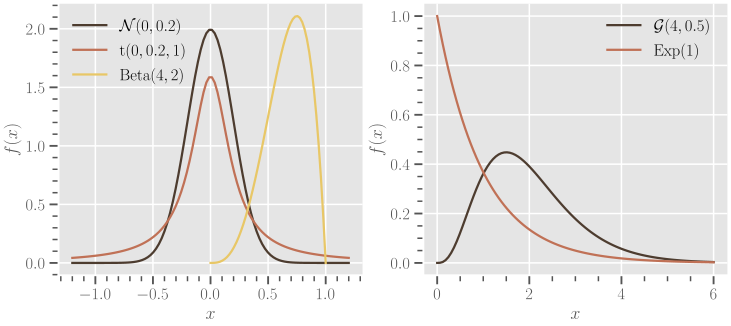
\includegraphics[width=\linewidth]{01_Rozklady_1D}
	\caption{\textbf{Jednowymiarowe zmienne losowe.} Przykładowe gęstości zmiennych losowych z tabeli \ref{tab:przykladowe_zmienne_losowe}.\label{fig:przykladowe_zmienne_losowe}}
\end{figure}

Do opisu zmiennych losowych \emph{wielo}wymiarowych, oprócz gęstości łącznej rozkładu wyróżniamy dodatkowo gęstości warunkowe i brzegowe. Opisują one jak zachowuje się współrzędna wektora losowego, jeśli pozostałe z nich przyjmą pewne wartości, lub jeśli kompletnie wyłączymy ich wpływ.

\begin{df}[Rozkłady brzegowy]
	Rozpatrzmy d-wymiarową zmienną losową $\mathbf{X} = [X_1, X_2, \dots, X_d]$ o gęstości $f(x_1, \dots, x_d)$. Gęstość rozkładu brzegowego $X_j$ definiujemy jako:
	$$f_j(x_j)=\int_{-\infty}^{\infty}\dots\int_{-\infty}^{\infty} f(x_1, \dots, x_{j-1}, x_j, x_{j+1}, \dots, x_d)  dx_1\dots dx_{j-1} dx_{j+1} \dots dx_d.$$
\end{df}

\begin{df}[Rozkład warunkowy]
	Rozpatrzmy d-wymiarową zmienną losową $\mathbf{X} = [X_1, X_2, \dots, X_d]$ o gęstości $f(x_1, \dots, x_d)$. Gęstość rozkładu warunkowego $X_j \vert X_k$ definiujemy jako:
	$$f_{j|k}(x_j|x_k) = \frac{f(x_1, \dots, x_d)}{f_k(x_k)}.$$
\end{df}


\section{Rozkłady wielowymiarowe}
\label{sec:rozklady_wielowymiarowe}
Naturalnym jest więc, że w praktyce często rozważamy modele wielowymiarowych zmiennych losowych, które mają regularne, łatwe do opisania gęstości łączne. Rozkłady jednowymiarowe z tabeli \ref{tab:przykladowe_zmienne_losowe} w naturalny sposób znajdują swoje rozszerzenia na więcej wymiarów (\cite{MultivariateDistributions}, \cite{Cherubini_Copula_Methods_in_Finance}). Najpopularniejszym tego przykładem jest rodzina $d$-wymiarowych rozkładów eliptycznych, do której należą rozkłady o gęstości postaci:

$$ f_{\mathcal{N}}(x, \mu, \Sigma) = k_d \vert\Sigma\vert^{-0.5}g\big((x-\mu)^T\Sigma^{-1}(x-\mu)\big).$$

W powyższej reprezentacji, $k_d \in\mathbb{R}$ jest stałą zależną od wymiaru, $\mu$ jest $d$-wymiarowym wektorem średnich, $\Sigma \in \mathbb{R}^{d \times d}$ to symetryczna, dodatnio zdefiniowana macierz, a $g \colon [0, \infty) \mapsto [0, \infty)$ jest pewną funkcją która nie zależy od wymiaru wektora.

Dla odpowiednio dobranych $g$ i $k_d$ otrzymamy w tej rodzinie wielowymiarowy rozkład normalny, czy wielowymiarowy rozkład t. Powstają one przy odpowiednio $k_d=(2\pi)^{-0.5d}$ i $g(s) = \exp(-0.5 t)$, lub $k_d=\Gamma(\frac{\nu + d}{2})/\Gamma(\frac{\nu}{2})$ i $g(s) = \big(1 + \frac{t}{\nu})^{-(\nu + d)/2}$.
\begin{figure}[H]
	\centering
	\includegraphics[width=0.45\linewidth]{01_MultivariateGaussian}	\includegraphics[width=0.45\linewidth]{01_MultivariateStudent}
	\caption{Gęstości przykładowych rozkładów eliptycznych ($d=2, \mu=[0, 0], \Sigma = \big[\begin{smallmatrix}2&1\\1&2\end{smallmatrix}\big]$). Lewy panel: $2$-wymiarowy rozkład normalny. Prawy panel: $2$-wymiarowy rozkład t ($\nu = 0.5$).\label{fig:multivariate_gaussian_student}}
\end{figure}

Używając rozkładów eliptycznych implikujemy model w którym rozkłady brzegowe pochodzą z tej samej rodziny. Obserwując rysunek \ref{fig:multivariate_gaussian_student}, można rozpoznać charakterystyczne kształty rozkładów brzegowych. Manipulując różnymi rozkładami eliptycznymi możemy więc zamodelować różne struktury korelacji między zmiennymi, czy też ciężkość ogonów, lecz tracimy swobodę wyboru rozkładów brzegowych. \cite{Markovitz_MPT} i jego model bazują właśnie na rozkładzie multinormalnym ponieważ zakładają, że wektor średnich i macierz korelacji wystarczająco opisuje rozkład zwrotów aktywów rynkowych. Podejście to łatwo obalić ze względu na empiryczne dowody ciężkoogonowego charakteru zachowania rynku akcji (\cite{Taleb_BS_is_BS}, \cite{Mandelbrot_NonGaussianity}), czy zjawiska niesymetrycznej, silniejszej korelacji w lewym ogonie (\cite{Taleb_BS_is_BS}, \cite{AssymetricEquityDependency}). Nie mniej jednak nie da się odmówić, że ten prosty model jest wystarczający aby uświadomić jak istotny jest wpływ zależności komponentów na zachowanie całego systemu.\\

\section{Miary współzależności}
\label{sec:miary_współzależności}
Problemem w poprawnym opisie zależności między zmiennymi losowymi jest fakt, że dostępnych mamy wiele statystyk które ją mierzą. Każda z nich uchwyca pewien konkretny aspekt współzależności, i nie da się jasno wyróżnić konkretnej jako "najlepszej". W tej sekcji pracy zaprezentujemy wybrane narzędzia służące do badania struktury zależności zmiennych losowych.

\subsubsection{$\rho$ Pearsona}
Podstawową i najbardziej znaną miarą współzależności zmiennych losowych jest korelacja Pearsona.

\begin{df}[Korelacja Pearsona]
	Niech $X$ i $Y$ będą zmiennymi losowymi o skończonych drugich momentach. Współczynnikiem korelacji pearsona $\rho$ nazywamy
	
	$$ \rho(X, Y) \coloneqq \Corr(X,Y) = \frac{\Cov(X,Y)}{\sqrt{\Var(X)}\sqrt{\Var(Y)}}.$$
\end{df}

Ten współczynnik korelacji przyjmuje wartości z zakresu $[-1, 1]$, gdzie $\vert\rho\vert=1$ oznacza idealną liniową relację. Korelacja pearsona jest podstawową miarą zależności podawaną w każdym podręczniku do statystyki. Ma jednak szereg wad: nie jest zdefiniowana dla ciężkoogonowych rozkładów (przez nieokreśloną wariancję), oraz jest wrażliwa na monotonicznie rosnące przekształcenia $X$ i $Y$. Te i wiele innych ograniczeń korelacji pearsona stoi w sprzeczności z aksjomatycznym podejściem do miar zgodności (czyt. \ref{def:miara_zgodnosci}). \\
Gdy w rozdziale \ref{subsec:dwuwymiarowe_kopuly_definicja} zdefiniujemy czym jest główny obiekt tej pracy, czyli kopuła, zależeć nam będzie, żeby móc opisać zależność zmiennych losowych $X$, $Y$ w terminach łączącej je kopuły $C$. Z tego powodu, interesujące dla nas będą miary zależności, które są niezmiennicze na monotonicznie rosnące przekształcenia (ze względu na transformację PIT \ref{def:PIT}, czyt. rozdział \ref{subsec:dwuwymiarowe_kopuly_definicja}). Korelacja pearsona nam tego nie zapewni, ale możemy zdefiniować inne miary: zgodności zmiennych losowych, które posiadają lepsze własności z punktu widzenia teorii kopuł.\\

Aby w pełni zdefiniować aksjomatyczne podejście do miar zgodności jak wprowadził to Scarsini w \cite{Scarsini1984}, potrzebujemy mieć dostępne pojęcie kopuły. W tej pracy formalnie zostaną one wprowadzone dopiero w definicji \ref{def:bivariate_copula}, w związku z czym na ten moment powiemy jedynie (nieformalnie), że kopuła jest funkcją która opisuje charakter i siłę zależności między zmiennymi losowymi. Pełną definicję i opis czym są kopuły można przeczytać w rozdziale \ref{sec:dwuwymiarowe_kopuly}.

\begin{df}[Miara zgodności]
	Rozpatrzmy zmienne losowe $X$ i $Y$ powiązane kopułą $C$. $M_{X,Y}=M_C$ nazwiemy miarą zgodności, wtedy i tylko wtedy gdy:
	\begin{enumerate}
		\item jest zdefiniowana dla dowolnych zmiennych $X$, $Y$
		\item jest relatywna, lub znormalizowana: $M_{X,Y}\in[-1,1]$
		\item jest symetryczna: $M_{X,Y}=M_{Y,X}$
		\item jeśli $X$ i $Y$ są niezależne, to $M_{X,Y}=0$
		\item $M_{-X,Y}=M_{X,-Y}=-M_{Y,X}$
		\item jest zbieżna, gdy kopuła jest punktowo zbieżna, tzn. jeśli $\{(X_n,Y_n)\}$ jest ciągiem ciągłych zmiennych losowych o kopułach $\{C_n\}$, oraz 
		$$ \lim\limits_{n\to\infty} C_n(u, v) =C(u, v)\text{, dla każdych }(u, v)\in[0,1]^2,$$
		to wtedy
		$$ \lim\limits_{n\to\infty}M_{X_n,Y_n}=M_{X,Y}.$$
		\item przestrzega relacji zgodności: jeśli $C_1(u,v) \leqslant C_2(u,v)$ dla wszystkich $(u, v)\in[0,1]^2$, to $M_{C_1} \leqslant M_{C_2}.$
	\end{enumerate}
	\label{def:miara_zgodnosci}		
\end{df}

Aksjomatyczne podejście z powyższej definicji zawęża przestrzeń miar zgodności do takich, które są niezmiennicze względem rosnących transformacji, czyli:
$$ M_{X,Y} = M_{\alpha(X), \beta(Y)},$$
dla dowolnych funkcji $\alpha,\beta$ rosnących prawie wszędzie.\\

\subsubsection{Współmonotoniczność i przeciwmonotoniczność}
Współmonotoniczność i przeciwmonotoniczność to szczególne przypadki zależności zmiennych losowych, w których są one od siebie perfekcyjnie zależne.

\begin{df}[Zbiór współmonotoniczny]
	Zbiór $A \subset \R^2$ nazywamy współmonotonicznym, wtedy i tylko wtedy gdy dla dowolnych $(x_1, y_1)$, $(x_2, y_2)$ z $A$ zachodzi:
	
	$$ (x_1 - y_1)(x_2 - y_2) >0.$$
\end{df}

\begin{df}[Zbiór przeciwmonotoniczny]
	Zbiór $A \subset \R^2$ nazywamy przeciwmonotonicznym, wtedy i tylko wtedy gdy dla dowolnych $(x_1, y_1)$, $(x_2, y_2)$ z $A$ zachodzi:
	
	$$ (x_1 - y_1)(x_2 - y_2) <0.$$
\end{df}


\begin{df}[Zmienne losowe współ- i przeciwmonotoniczne]
	Wektor losowy $(X, Y)$ nazywamy współmonotonicznym (przeciwmonotonicznym), lub perfekcyjnie dodatnio (ujemnie) zależnym wtedy i tylko wtedy gdy istnieje zbiór współmonotoniczny (przeciwmonotoniczny) $A\subset\R^2$:
	
	$$ \Pra[(X,Y)\in A]=1.$$
\end{df}

Współmonotoniczność i przeciwmonotoniczność zmiennych losowych jest ważnym konceptem w teorii kopuł, ponieważ definiuje najsilniejszy rodzaj zależności jakie kopuły mogą reprezentować (czyt. twierdzenie \ref{thm:frechet_hoeffding}).

\subsubsection{$\tau$ Kendalla i $\rho$ Spearmana}

Współczynniki $\tau$ Kendalla i $\rho$ Spearmana oba spełniają aksjomaty miar zgodności z \cite{Scarsini1984}. Są współczynnikami rangowymi, więc nie zależą od monotonicznych przekształceń rozkładów brzegowych $X$ czy $Y$. Ich zaletą jest to, że mogą być przez to jednoznacznie przedstawione w języku kopuły - co znajduje zastosowanie przy estymacji parametrów modeli kopułowych. Ta własność zazwyczaj nie zachodzi w przypadku korelacji Pearsona.

\begin{df}[$\tau$ Kendalla]
	Współczynnik $\tau$ Kendalla między ciągłymi zmiennymi losowymi $X$ i $Y$ o kopule definiujemy jako:
	$$ \tau = \Pra[(X_1-X_2)(Y_1-Y_2)>0] - \Pra[(X_1-X_2)(Y_1-Y_2) <0], $$
	gdzie $(X_1, Y_1)$ i $(X_2, Y_2)$ są kopiami iid wektora $(X, Y)$.
\end{df}

\begin{df}[$\rho$ Spearmana]
	Współczynnik $\rho$ Spearmana między ciągłymi zmiennymi losowymi $X$ i $Y$ o rozkładach brzegowych $F_X$ i $F_y$ zadany jest przez:
	$$ \rho = \Corr[F_X(X), F_Y(Y)].$$
\end{df}

Współczynniki te dają się jednoznacznie wyrazić za pomocą kopuł łączących $X$~i~$Y$~-~własność tę podamy w rozdziale \ref{subsec:dwuwymiarowe_kopuly_definicja}. Istotny również jest fakt, że ich ekstremalne wartości, tj. $\rho= 1$, czy $\tau=1$ odpowiadają współmonotoniczności zmiennych losowych, a $\rho=-1$, czy $\tau=-1$ odpowiadają przeciwmonotoniczności.

\subsubsection{Zależność ogonów}
Na zależność zmiennych losowych można popatrzeć również ze strony zależności obserwacji ekstremalnych. Rozważmy następującą statystykę:

\begin{df}[Współczynnik zależności ogonów]
	Górnym współczynnikiem zależności ogonów $(X_1, X_2)$ o rozkładach brzegowych $F_1$ i $F_2$ i kopuli $C$ nazywamy:
	$$ \lambda^{u} = \lim\limits_{t\to1^{-}}\Pra[X_2 > F_2^{-1}(t) \vert X_1 > F_1^{-1}(t) ].$$
	Dolnym współczynnikiem nazywamy:
	$$ \lambda^{l} = \lim\limits_{t\to0^{+}}\Pra[X_2 \leqslant F_2^{-1}(t) \vert X_1 \leqslant F_1^{-1}(t) ].$$
\end{df}

Współczynniki zależności ogonów informują o sile zależności zmiennych losowych w granicy, gdy dążymy z jedną z nich coraz dalej w jej ogon. Mówimy, że zmienne losowe posiadają zależność ogonów jeśli $\lambda \in (0, 1]$, lub jej nie posiadają gdy $\lambda =0$. Te wspołczynniki zależą przede wszystkim od obserwacji będących ekstremalnymi względem obu zmiennych. Rysunek \ref{fig:tail_dependence} prezentuje przykładowy rozkład posiadający dolny współczynnik zależności ogonów, lecz nie posiadający górnego wspołczynnika. Kolorami zaznaczone są obserwacje które wpływają na dolny (szare punkty) i górny (czerwone punkty) współczynnik zależności ogonów.\\
W praktycznych zastosowaniach, jest on jednak trudny do kalibracji z danych - koncept ten działa raczej w drugą stronę: z parametrów skalibrowanego modelu implikowany jest współczynnik zależności ogonów.
\begin{figure}[H]
	\centering
	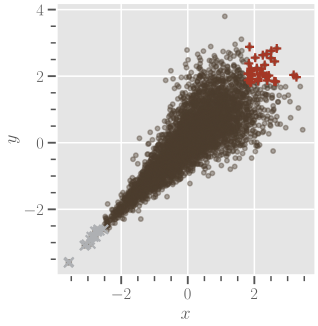
\includegraphics[width=0.5\linewidth]{01_Tail_dependence}	
	\caption{Ilustracja górnego i dolnego współczynnika zależności ogonów.\label{fig:tail_dependence}}
\end{figure}

W tym rozdziale zdefiniowialiśmy różne miary pomagające nam zrozumieć zależność zmiennych losowych. Widzimy zatem, że korelacja Pearsona i modele eliptyczne to za mało, aby w pełni uchwycić charakter współzależności. W kolejnym rozdziale podamy teorię \emph{kopuł}, które dadzą nam odpowiednie narzędzia do walki z tym problemem.


\mgrclosechapter
\chapter{Modele kopułowe}
\label{ch:modele_kopulowe}
Zgodnie z drugim filarem Basel II instytucje finansowe zobowiązane są dokonywać regularnych symulacji stress testowych, podczas których ich kondycja finansowa poddawana jest ekstremalnym negatywnym ruchom rynkowym. Ma to na celu postawienie instytucji przed hipotetycznym kryzysowym scenariuszem i ocenę czy instytucja ma zgromadzoną wystarczającą ilość kapitału ekonomicznego aby przetrwać taką sytuację (\cite{BaselII}). Podczas symulacji stress testowych, regulator podaje instytucjom ogólny scenariusz rynkowy w postaci trajektorii pewnych wiodących zmiennych makroekonomicznych. Każda instytucja musi następnie zinterpretować zadany scenariusz i rozszerzyć go na zbiór zmiennych istotnych z punktu widzenia ich biznesu. Standardową praktyką w tym procesie, nazywanym \emph{shock expansion}, wciąż są modele ekonometryczne, wynikiem których są w większości pojedyncze trajektorie. \cite{Siddique_Stress_testing}\\
Podejście to ma istotną wadę: nie jesteśmy w nim w stanie podać prawdopodobieństwa wystąpienia takiej realizacji \emph{shock expansion}, ponieważ wynikiem są jedynie pojedyncze trajektorie. Nowym kierunkiem w procesie \textit{shock expansion} zaczyna być natomiast tzw. probabilistic stress testing (np. \cite{Aste_Probabilistic_Stress_Testing}). Ideą jest tu zamodelowanie wielowymiarowego systemu zmiennych makroekonomicznych i rynkowych, w sposób pozwalający zaaplikowanie rynkowej narracji regulatora jako zbioru warunkującego ten system. Umożliwia to odzyskanie rozkładów warunkowych dla innych komponentów systemu, w szczególności dla tych które są potrzebne jako wynik \emph{shock expansion}.\\
\cite{Aste_Probabilistic_Stress_Testing} w swojej pracy bada potencjalne zastosowanie rozkładów eliptycznych, wprowadzonych w rozdziale \ref{sec:rozklady_laczne} jako jednego, wielowymiarowego modelu wyżej opisanego systemu. Wyniki które otrzymuje wskazują, że mimo iż rozkłady eliptyczne dają intuicyjne wyniki co do ogólnego kierunku rozwoju warunkowanych rozkładów, to nie są wystarczająco elastyczne aby poprawnie uchwycić wszystkie cechy systemu. Jako tego powód, Aste wymienia \textit{symetrię} modelu, która przejawia się w konieczności wyboru tych samych rodzin rozkładów brzegowych i jest implikowana użyciem rozkładów eliptycznych.\\

Powyższy przykład to jeden z długiego szeregu który ilustruje, że praktyczne problemy wymagają dowolności w wyborze rozkładów brzegowych (wiele innych interesujących przykładów podają \cite{Cherubini_Copula_Methods_in_Finance}, czy \cite{Cherubini_Dynamic_Copula_Methods_in_Finance}). Dlatego mimo, że istnieje wiele matematycznie poprawnych rozszerzeń zmiennych losowych z $d=1$ do $d>2$ (jak wielowymiarowy rozkład normalny, wielowymiarowy rozkład t-Studenta, wielowymiarowy rozkład gamma, etc.), to nie cieszą się one dużym zastosowaniem w praktyce. Odpowiedzią na to ograniczenie są kopuły - modele wielowymiarowych zmiennych losowych, pozwalające na oddzielenie wpływu rozkładów brzegowych od wpływu struktury zależności na cały system.\\

\section{Dwuwymiarowe kopuły}
\label{sec:dwuwymiarowe_kopuly}
\subsection{Wprowadzenie i definicja}
Teorię kopuł zapoczątkował Abe Sklar w \cite{Sklar_Theorem}, podając następujące twierdzenie:

\begin{thm}[Twierdzenie Sklara]
	Niech $X_1, X_2, \dots, X_d$ będą zmiennymi losowymi ciągłymi, o dystrybuantach $F_1, \dots, F_d$, i rozkładzie łącznym z dystrybuantą $F$. Wtedy istnieje dokładnie jedna \emph{kopuła} $C$, taka że dla wszystkich $\mathbf{x} = (x_1, \dots, x_d) \in \mathbb{R}^d$:
	\begin{equation}
		F(x_1, \dots, x_d) = C(F_1(x_1), \dots, F_d(x_d)).
		\label{eq:sklar_theorem}
	\end{equation}
	
	Zachodzi również twierdzenie odwrotne: Mając dowolne dystrybuanty $F_1, \dots, F_d$ i kopułę $C$, funkcja $F$ zdefiniowana według \ref{eq:sklar_theorem} jest d-wymiarową dystrybuantą, o rozkładach brzegowych $F_1, \dots, F_d$. 
	\label{thm:sklar_theorem}
\end{thm}

Twierdzenie \ref{thm:sklar_theorem} przede wszystkim podaje więc algorytm postępowania mówiący w jaki sposób otrzymać wielowymiarowy rozkład o dowolnie wybranych, potencjalnie różnych rozkładach brzegowych. Dodatkowo, Sklar stwierdza istnienie pewnego obiektu, nazwanego kopułą/funkcją łączącą (łac.\emph{copulae}: łączyć) który jest jednoznacznie zdefiniowany dla dowolnego ciągłego rozkładu wielowymiarowego, w taki sposób, że rozkład łączny da się przedstawić jako tę funkcję zaaplikowaną do rozkładów brzegowych.\\

Oczywistym jest, że nie wszystkie wielowymiarowe funkcje mogą pełnić taką rolę. Rozważymy więc jakie warunki musi spełniać $C$ z twierdzenia \ref{thm:sklar_theorem}, aby mogła być kopułą.
\begin{df}[Grounded function]
	Rozważmy $A_1$ i $A_2$ - dwa niepuste podzbiory $\mathbb{R}$, oraz funkcję $G\colon A_1\times A_2\mapsto\mathbb{R}$. Niech $a_i$ oznacza najmniejszy element $A_i$, dla $i=1, 2$. Funkcję $G$ będziemy nazywać uziemioną (\emph{grounded}), jeśli dla każdej pary $(v, z)$ z $A_1\times A_2$,
	\begin{equation}
		G(a_1, z) = 0 = G(v, a_2).
	\end{equation}
	\label{def:grounded_function}
\end{df}

\begin{df}[2-increasing function]
	$G\colon A_1\times A_2\mapsto \mathbb{R}$ nazywamy dwu-rosnącą (\emph{2-increasing}), jesli dla każdego prostokąta $[v_1, v_2]\times [z_1, z_2]$ $(v_1 \leqslant v_2$, $z_1\leqslant z_2)$ którego wierzchołki leżą w $A_1 \times A_2$ mamy
	\begin{equation}
		G(v_2, z_2) - G(v_2, z_1) - G(v_1, z_2) + G(v_1, z_1) \geqslant 0.
	\end{equation}
	\label{def:two_increasing_function}
\end{df}

Definicje \ref{def:grounded_function} oraz \ref{def:two_increasing_function} pozwalają na poprawne zdefiniowanie kopuły:
\begin{df}[Dwuwymiarowa kopuła]
	Dwuwymiarową kopułą $C$ nazwiemy funkcję rzeczywistą zdefiniowaną na kwadracie jednostkowym:
	$$ C\colon [0, 1]\times[0, 1] \mapsto \mathbb{R},$$ o następujących własnościach:
	\begin{itemize}
		\item uziemiona $\big(C(v, 0) = 0 = C(0, z)\big)$
		\item dwu-rosnąca
		\item $C(v, 1) = v$ oraz $C(1, z) = z$ dla wszystkich $(v, z)\in [0,1]\times [0, 1].$
	\end{itemize}
	\label{def:bivariate_copula}
\end{df}

Aby zrozumieć czym kopuła tak naprawdę jest warto wrócić do twierdzenia \ref{thm:sklar_theorem}. Równość \ref{eq:sklar_theorem} implikuje, że kopuła musi być dystrybuantą pewnego wielowymiarowego rozkładu. Definicja kopuły w \ref{def:bivariate_copula} mówi natomiast, że ta dystrybuanta jest zdefiniowana na \emph{kwadracie jednostkowym}. Kopuła jest więc niczym innym jak dystrybuantą wielowymiarowego rozkładu jednostajnego. Istotnie: można pokazać, że argumenty kopuli w równaniu \ref{eq:sklar_theorem} mają rozkład jednostajny, co udowadniamy poniżej i ilustrujemy na rysunku \ref{fig:PIT}.

\begin{df}[Probability integral transform]
	Jeśli $X\sim F$ jest ciągłą zmienną losową, a $x$ jest jej realizacją, to transformację $u\coloneqq F(x)$ nazywamy \emph{probability integral transform} (PIT) w punkcie $x$.
	\label{def:PIT}
\end{df}
\begin{thm}[Probability integral transform]
	Jeśli $X\sim F$ jest ciągłą zmienną losową, to $U\coloneqq F(X)$ ma rozkład jednostajny.
\end{thm}
\begin{proof}
	$$P(U\leqslant u) = P(F(X) \leqslant u) = P(X\leqslant F^{-1}(u))=F(F^{-1}(u))=u.$$
\end{proof}

\begin{figure}[H]
	\centering
	\includegraphics[width=0.6\linewidth]{01_PIT}	
	\caption{\textbf{Probability Integral Transform. } Ilustracja działania PIT. Zmienna losowa z rozkładu lognormalnego $
		\mathcal{LN}(0.5, 1)$ (pozioma oś) przekształcana jest przez własną dystrybuantę do rozkładu jednostajnego $\mathcal{U}(0, 1)$ (pionowa oś).\label{fig:PIT}}
\end{figure}

Wróćmy na chwilę do oryginalnego pytania, czyli modelowania wielowymiarowych zmiennych losowych. Na początku rozdziału zdefiniowaliśmy kopułę jako funkcję spełniającą równanie \ref{eq:sklar_theorem} z twierdzenia Sklara, czyli:
$$F(x_1, \dots, x_d) = C(F_1(x_1), \dots, F_d(x_d)).$$

Prawą stronę równania stanowią wyizolowane rozkłady brzegowe, oraz pewna funkcja $C$, postać której jest kompletnie od nich niezależna. Lewa strona równania, to natomiast rozkład łączny pewnej zmiennej losowej. Jeśli zastanowimy się co wpływa na charakter rozkładu łącznego zmiennej losowej, dojdziemy do wniosku, że istnieją dwa komponenty: zachowanie rozkładów brzegowych, oraz ich współzależności. Biorąc znów pod uwagę prawą stronę równania, kopuła musi więc odpowiadać za współzależności między rozkładami brzegowymi. \\
Istotnie, kopuły pozwalają na rozdzielenie problemu modelowania rozkładu łącznego, na modelowanie osobno rozkładów brzegowych, a osobno struktury ich współzależności (\cite{Sklar_Theorem}, \cite{Joe_Multivariate_Models}). Ta pozorna prostota tworzenia wielowymiarowych modeli przyczyniła się do szybkiej ich popularyzacji, ale i przyniosła ze sobą duże ryzyko modelu. Najbardziej znanym tego przykładem jest zapewne fiasko modeli wyceniających produkty typu CDO (\cite{CDS_Copula}), które niedoszacowywały nasilenia korelacji bankructw wewnątrz struktury tego kontraktu.\\

Zauważamy zatem dualizm kopuł - można patrzeć na nie zarówno jak na funkcje łączące ze sobą dowolne rozkłady brzegowe w spójny rozkład łączny lub też jak na dystrybuanty wielowymiarowych rozkładów jednostajnych.\\
\label{subsec:dwuwymiarowe_kopuly_definicja}

\subsection{Probabilistyczna interpretacja}
Przyjrzymy się więc jednej stronie powyższego dualizmu i przeanalizujmy kopuły jako struktury zależności.

\begin{df}[Kopuła minimum]
	Dwuwymiarowa kopuła minimum $C^{-}$ to kopuła zadana wzorem $C^{-}(u, v) = \max(u+v-1, 0).$
\end{df}
\begin{df}[Kopuła maximum]
	Dwuwymiarowa kopuła maksimum $C^{+}$, to kopuła zadana wzorem $C^{+}(u, v) = \min(u, v).$
\end{df}

\begin{figure}[h]
	\centering
	\includegraphics[width=0.35\linewidth]{01_MaximumCopula_contour}
	\includegraphics[width=0.4\linewidth]{01_MaximumCopula_surface}
	\includegraphics[width=0.35\linewidth]{01_IndependenceCopula_contour}
	\includegraphics[width=0.4\linewidth]{01_IndependenceCopula_surface}
	\includegraphics[width=0.35\linewidth]{01_MinimumCopula_contour}
	\includegraphics[width=0.4\linewidth]{01_MinimumCopula_surface}
	
	\caption{Dystrybuanty (po lewej) i kontury (po prawej) kopuł: maximum (górny panel), produktowej (panel środkowy) i minimum (dolny panel)\label{fig:minmaxprod_copula}}
\end{figure}

Powyższe kopuły stanowią horyzont osiągalnych kopuł, ponieważ jak mówi twierdzenie \ref{thm:frechet_hoeffding}, są one ograniczeniem dolnym i górnym dla dowolnej innej kopuli. Ich powierzchnie i kontury przedstawia rysunek \ref{fig:minmaxprod_copula}. 

\begin{thm}[Fréchet-Hoeffding bounds]
	Niech $C$ będzie $2$-wymiarową kopułą. Wtedy dla każdego $(u, v)\in[0, 1]^2$ zachodzi
	
	$$ C^{-}(u, v) \leqslant C(u, v) \leqslant C^{+}(u, v).$$
	
	\label{thm:frechet_hoeffding}
\end{thm}

Twierdzenie to, choć z pozoru teoretyczne, ciągnie za sobą bardzo praktyczne konsekwencje: pozwala otrzymać niezależne od modelu ogranicznia górne i dolne na dowolną kopułę. \cite{Cherubini_Copula_Methods_in_Finance} pokazuje przykład, gdzie twierdzenie Frécheta-Hoeffdinga pozwala na uzyskanie dolnego i górnego ograniczenia na pewne statystyki modelu, jak np. łączne prawdopodobieństwo bankructwa dwóch firm w strukturalnym modelu Mertona, czy cena opcji binarnej na dwa aktywa.

\begin{df}[Kopuła produktowa]
	Dwuwymiarowa kopuła produktowa $C^{\perp}$ to kopuła zadana wzorem $C^{\perp}(u, v) = uv.$
\end{df}

Kopuła produktowa jest trzecim istotnym punktem odniesienia w świecie kopuł, ponieważ posiada pewną unikalną właśność. Z jednej strony z definicji kopuły mamy:

\begin{equation}
C(u, v) = P(U \leqslant u, V \leqslant v )
\label{eq:independence_copula1}
\end{equation}

Z drugiej jednak strony, wiemy że $U$ i $V$ mają rozkłady jednostajne - więc:
\begin{equation}
	F_U(u) = P(U \leqslant u) = u\text{, oraz } F_V(v) = P(V \leqslant v) = v.
\label{eq:independence_copula2}
\end{equation}

Z równań \ref{eq:independence_copula1} i \ref{eq:independence_copula2}, dla przypadku kopuły produktowej mamy zatem:
\begin{equation}
	P(U \leqslant u, V \leqslant v ) \equiv C^{\perp}(u, v) = uv = P(U \leqslant u) P(V \leqslant v).
	\label{eq:independence_copula}
\end{equation}

Równanie \ref{eq:independence_copula} mówi nam, że zmienne losowe $V$ i $U$ są od siebie niezależne. Model kopuły produktowej, implikuje więc niezależność jednostajnych rozkładów brzegowych.
Co więcej, uzupełniając opis kopuł minimum i maksimum - te z kolei odpowiadają współmonotonicznej \emph{(eng. comonotone)} i przeciwmonotonicznej \emph{(eng. countermonotone)} zależności jednostajnych rozkładów brzegowych. Zgodnie z twierdzeniem \ref{thm:frechet_hoeffding} natomiast wszystkie inne kopuły modelują pozostałe rodzaje zależności istniejące pomiędzy tymi ekstremami. Widzimy więc, że kopuły potrafią modelować pełne spektrum możliwych zależności: od współmonotonicznych, przez niezależne, aż po przeciwmonotoniczne. 
\label{subsec:dwuwymiarowe_kopuly_probal}

\subsection{Popularne kopuły i ich własności}
Rozdział \ref{subsec:dwuwymiarowe_kopuly_probal} pokazał, że kopuły można intuicyjnie rozumieć jako modele zależności. W tej sekcji spojrzymy na nie z dualnej perspektywy, jako na dystrybuanty, co pozwoli nam zdefiniować użyteczne narzędzia do analizy charakteru tej zależności.

\begin{df}[Gęstość kopuły]
	Niech $C$ będzie $d$-wymiarową (jednostajnie ciągłą) kopułą. Gęstością tej kopuły nazywamy funkcję
	\begin{equation}
		c(u_1, \dots, u_d) = \frac{\partial^d}{\partial u_1\dots \partial u_d}C(u_1, \dots, u_d).
		\label{eq:copula_density}
	\end{equation}
\end{df}


Widzimy, że równanie \ref{eq:copula_density} jest jedynie przeniesieniem terminu gęstości wielowymiarowego rozkładu na grunt kopuł. Zanim zaczniemy wizualizować gęstości konkretnych kopuł, warto wspomnieć, że Sklar w \cite{Sklar_Theorem} podaje również alternatywną wersję swojego twierdzenia o istnieniu kopuły, tym razem w języku gęstości. Sens i zastosowania twierdzenia pozostają takie same jak dla twierdzenia \ref{thm:sklar_theorem}.
\begin{thm}[Twierdzenie Sklara: gęstość kopuły]
	Niech $X$ będzie $d$-wymiarowym wektorem losowym o dystrybuancie rozkładu łącznego $F$, oraz rozkładami brzegowymi $F_i$, $i=1, \dots, d$. Wtedy rozkład łączny może być wyrażony jako		$$F(x_1, \dots, x_d) = C(F_1(x_1), \dots, F_d(x_d)),$$
	lub równoważnie w terminach gęstości poprzez:
	$$ f(x_1, \dots, x_d) = c(F_1(x_1), \dots, F_d(x_d))\cdot f_1(x_1)\dots f_d(x_d),$$
	dla pewnej $d$-wymiarowej kopuli $C$, o gęstości $c$. Dla rozkładów bezwzględnie ciągłych, kopuła $C$ jest jednoznacznie określona.\\
	Zachodzi również twierdzenie odwrotne: kopuła związana z wielowymiarowym rozkładem $F$ o rozkładach brzegowych $F_1, \dots F_d$ może być wyrażona jako:
	$$C(u_1, \dots, u_d) = F(F_1^{-1}(u_1), \dots, F_d^{-1}(u_d)),$$
	a jej gęstość wyraża się poprzez:
	$$c(u_1, \dots, u_d) = \frac{f(F_1^{-1}(u_1), \dots, F_d^{-1}(u_d))}{f_1(F_1^{-1}(u_1))\dots f_d(F_d^{-1}(u_d))}$$
	\label{thm:sklar_theorem_density}
\end{thm}

Resztę rozdziału stanowić będzie omówienie różnych rodzin kopuł o istotnych zastosowaniach w praktyce. Będziemy prezentować ich gęstości, ponieważ w intuicyjny sposób przedstawiają one mapę osłabień i nasileń współzależności dla konkretnych kopuł. Informatywne w tym względzie są ich wykresy konturowe, przedstawiające izohipsy powierzchni gęstości. Standardowo przedstawia się je w naturalnej \emph{skali kopuły}, tzn. na kwadracie jednostkowym wizualizuje się bezpośrednio gęstość kopuły:
$$ c(u, v)\text{, dla } (u, v) \in [0, 1]^2.$$
Pomocna jest jednak również wizualizacja w \emph{skali brzegowo-znormalizowanej}, czyli po dokonaniu transformacji przez dystrybuantę $\Phi$ i gęstość $\phi$ standardowego rozkładu normalnego:
 $$ g(x, y) = c(\Phi(x), \Phi(y))\phi(x)\phi(y)\textit{, dla }(x,y)\in\R^2.$$
Powyższa transformacja nie wizualizuje już gęstości kopuły $c$, ale raczej gęstość rozkładu wielowymiarowego $g$, który powstałby gdybyśmy kopułą $c$ połączyli zmienne ze standardowego rozkładu normalnego, zgodnie z twierdzeniem \ref{thm:sklar_theorem}. Ta reprezentacja jest bardzo intuicyjna, ponieważ podstawowe kursy statystyki przyzwyczajają ludzkie oko do utożsamiania silnej/słabej korelacji z wydłużonymi/okrągłymi elipsami tworzonymi przez gęstość wielowymiarowego rozkładu normalnego. Reprezentacja w skali brzegowo-znormalizowanej jest intuicyjna, ponieważ dla kopuły gaussowskiej pokazuje dokładnie te same, znane elipsy. Natomiast w przypadku innych kopuł, obserwujemy rozbieżność izohips od eliptycznego kształtu co daje się łatwo zinterpretować. 

W praktyce istnieją trzy główne nurty tworzenia kopuł. Można wykorzystać do tego twierdzenie Sklara \ref{thm:sklar_theorem} jako twierdzenie konstrukcyjne, tj. wziąć pewien istniejący, znany rozkład wielowymiarowy, zaaplikować \emph{PIT} (\ref{def:PIT}) do jego rozkładów brzegowych i odzyskać w ten sposób $C$ z twierdzenia Sklara. Drugą metodą konstrukcji kopuł jest zdefiniowanie ich przez tzw. \emph{generator} - powstają w ten sposób kopuły archimedejskie. Trzeci sposób natomiast to rozszerzenie \emph{extreme-value theory} z jedego do wielu wymiarów, co skutkuje powstaniem kopuł typu \emph{extreme-value}.\\

\underline{Rodzina kopuł eliptycznych}
\vspace{0.5cm}

Kopuły eliptyczne są przykładem konstrukcji kopuł poprzez bezpośrednią aplikację twierdzenia Sklara \ref{thm:sklar_theorem} do rozkładów eliptycznych, zdefiniowanych na początku rozdziału \ref{sec:rozklady_wielowymiarowe}. Można więc tę konstrukcję rozumieć jako implikowanie struktury zależności z wielowymiarowych rozkładów, poprzez wyeliminowanie wpływu rozkładów brzegowych. W tej rodzinie zobaczymy przede wszystkim kopuły reprezentujące zależności "implikowane" z wielowymiarowego rozkładu normalnego, czy wielowymiarowego rozkładu $t$.

\begin{df}[Kopuła produktowa]
	Kopuła produktowa to kopuła o gęstości:
	
	$$ c(u_1, u_2) = 1.$$
	
\end{df}
\begin{figure}[h]
	\centering
	\begin{minipage}{0.5\linewidth}
		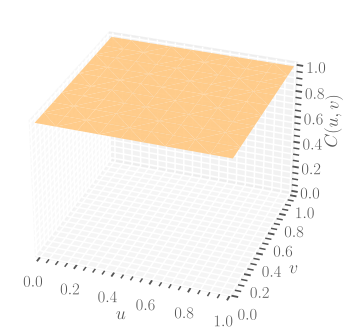
\includegraphics[width=\linewidth]{02_IndependenceCopula_density}
	\end{minipage}
	\begin{minipage}{0.45\linewidth}
		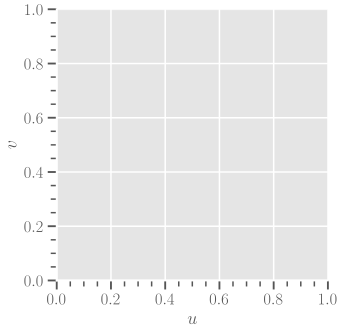
\includegraphics[width=.8\linewidth]{02_IndependenceCopula_contour}
		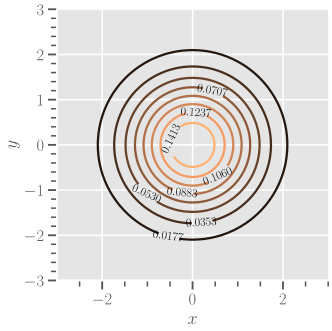
\includegraphics[width=.8\linewidth]{02_IndependenceCopula_contour_norm}
	\end{minipage}
	\caption{Gęstość kopuły produktowej: powierzchnia (lewy panel), kontur w skali kopuły (prawy górny panel), kontur w skali brzegowo-znormalizowanej (prawy dolny panel). \label{fig:product_copula_density}}
\end{figure}

Dystrybuantę tej kopuły przedstawiliśmy wcześniej na rysunku \ref{fig:prod_copula}, jednak w tym rozdziale pokazujemy ją w nieco innym świetle. Jednakowa gęstość widoczna na rysunku \ref{fig:product_copula_density} w każdym punkcie kwadratu jednostkowego mówi, że każda para $(u, v) \in [0,1]^2$ ma jednakową szansę na występienie, więc nie ma żadnej zależności między $U$ a $V$. Jest to zgodne z uwagą z rozdziału \ref{subsec:dwuwymiarowe_kopuly_probal}, mówiącą że ta kopuła odpowiada niezależnemu połączeniu zmiennych losowych. Zwróćmy uwagę na prawy dolny panel rysunku \ref{fig:product_copula_density}, który prezentuje izohipsy w skali brzegowo-znormalizowanej. Widzimy koncentryczne okręgi, kojarzące się z wielowymiarowym rozkładem normalnym o korelacji $0$. Istotnie, kopuła produktowa reprezentuje strukturę zależności w tym wielowymiarowym rozkładzie.

\begin{df}[Kopuła gaussowska]
	Kopuła gaussowska o korelacji $\rho$, to kopuła zadana wzorem:
	
	$$ C(u_1, u_2; \rho) = \Phi_2(\Phi^{-1}(u_1), \Phi^{-1}(u_2);\rho),$$
	
	gdzie $\Phi$ oraz $\phi$ to odpowiednio dystrybuanta i gęstość standardowego rozkładu normalnego. Gęstość kopuły gaussowskiej zadana jest wzorem:
	$$ c(u_1, u_2; \rho) = \frac{1}{\phi(x_1)\phi(x_2)} \frac{1}{\sqrt{1-\rho^2}}\exp\bigg[-\frac{\rho^2(x_1^2+x_2^2) - 2\rho x_1 x_2}{2(1-\rho^2)}\bigg],$$
	gdzie $x_i\coloneqq \Phi^{-1}(u_i)$.
\end{df}
\begin{figure}[h]
	\centering
	\begin{minipage}{0.5\linewidth}
		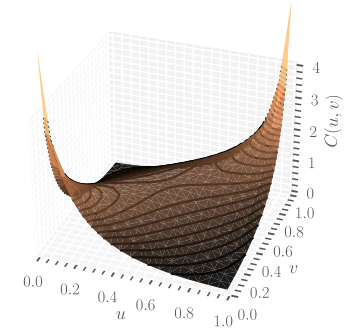
\includegraphics[width=\linewidth]{02_GaussianCopula_density}
	\end{minipage}
	\begin{minipage}{0.45\linewidth}
		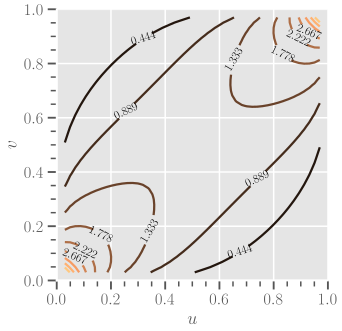
\includegraphics[width=.8\linewidth]{02_GaussianCopula_contour}
		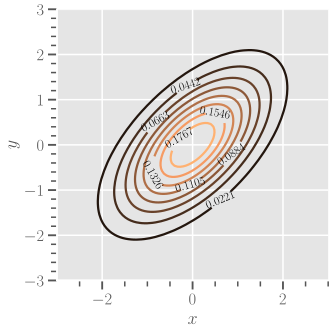
\includegraphics[width=.8\linewidth]{02_GaussianCopula_contour_norm}
	\end{minipage}
	\caption{Gęstość kopuły gaussowskiej, $\rho=0.6$: powierzchnia (lewy panel), kontur w skali kopuły (prawy górny panel), kontur w skali brzegowo-znormalizowanej (prawy dolny panel). \label{fig:gaussian_copula_density}}
\end{figure}

Kopuła gaussowska modeluje strukturę zależności implikowaną przez wielowymiarowy rozkład normalny, tj. wielowymiarowy rozkład normalny jest równoważny modelowi o normalnych rozkładach brzegowych, połączonych kopułą gaussowską. Rodzina kopuł gaussowskich jest wyczerpująca. Przykładowa powierzchnia gęstości oraz kontury kopuły gaussowskiej przedstawione są na rysunku \ref{fig:gaussian_copula_density}.

\begin{df}[Kopuła studenta]
	Kopuła studenta to jednoparametryczna kopuła o $\nu$ stopniach swobody i korelacji $\rho$ zadana jest gęstością:
	
	$$ C(u_1, u_2;\nu,\rho) = \frac{t(T_{\nu}^{-1}(v_1), T_{\nu}^{-1}(v_2);\nu,\rho)}{t_{\nu}(T_{\nu}^{-1}(v_1))t_{\nu}(T_{\nu}^{-1}(v_2))}.$$
\end{df}
\begin{figure}[h]
	\centering
	\begin{minipage}{0.5\linewidth}
		\includegraphics[width=\linewidth]{02_StudentCopula_density}
	\end{minipage}
	\begin{minipage}{0.45\linewidth}
		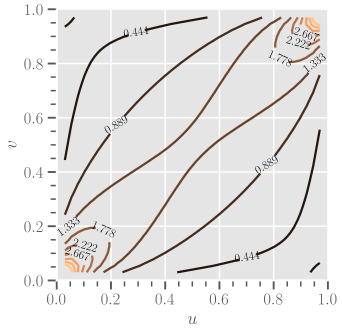
\includegraphics[width=.8\linewidth]{02_StudentCopula_contour}
		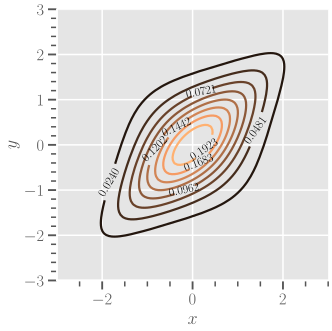
\includegraphics[width=.8\linewidth]{02_StudentCopula_contour_norm}
	\end{minipage}
	\caption{Gęstość kopuły studenta, $\nu=3, \rho=0.5$: powierzchnia (lewy panel), kontur w skali kopuły (prawy górny panel), kontur w skali brzegowo-znormalizowanej (prawy dolny panel). \label{fig:student_copula_density}}
\end{figure}
Kopuła studenta, podobnie do gaussowskiej, jest implikowana z rozkładu eliptycznego studenta. Oznacza to, że wielowymiarowy rozkład studenta jest równoważny modelowi o rozkładach brzegowych $t$ połączonych kopułą studenta. Wraz z rosnącą ilością stopni swobody kopuła studenta zbiega do gaussowskiej. Ta rodzina nie jest jednak wyczerpująca, ponieważ nawet przy $\rho=0$, dla żadnej skończonej liczby stopni swobody nie zawiera w sobie $C^{\perp}$.\\

Kopuły eliptyczne cieszą się dużą popularnością w instytucjach finansowych, ponieważ mają swoje naturalne $d$-wymiarowe rozszerzenia. Kopuły uważane są mimo wszystko za skomplikowane modele, i w obliczu szczegółowych regulacji nakładanych na wewnętrzne modele (np. w podejściu AMA do modelowania ryzyka operacyjnego \cite{BaselII}) dużo łatwiej jest uzasadnić i utrzymać w produkcji model bazujący na kilku intuicyjnych parametrach. Z tego powodu, kopuła $t$ studenta jest najczęściej wybieraną w praktyce - pozwala bowiem na modelowanie ciężkich ogonów i korelacji, a jednocześnie jest zaledwie dwuparametryczna (\cite{OpRisk}).\\

\underline{Rodzina kopuł archimedejskich}
\vspace{0.5cm}
\begin{df}[Kopuły archimedejskie]
		Niech $\mathcal{F}$ będzie zbiorem ciągłych, jednostajnie malejących i wypukłych funkcji $\phi \colon [0,1] \mapsto [0, \infty]$, takich, że $\phi(1) = 0$. Wtedy
		
		$$ C(u_1, u_2) = \phi^{[-1]}(\phi(u_1)+\phi(u_2))$$
		jest kopułą. Uściślając, nazwiemy ją kopułą archimedejską o generatorze $\phi$. W powyższej definicji, przez $\phi^{[-1]}$ rozumiemy pseudoodwrotność $\phi$, czyli funkcję $\phi^{[-1]}\colon [0, \infty] \mapsto [0, 1]$ zadaną przez:
		
		$$ \phi^{[-1]}(t) \coloneqq \phi^{-1}(t) \1_{\{0\leqslant t \leqslant \phi(0)\}}. $$
\end{df}

Ta rodzina została wprowadzona została przez Claytona w \cite{Clayton1972} w kontekście modelowania zapadalności na choroby przewlekłe, gdzie posłużyła do opisania zależności w aktuarialnych tabelach średniego dalszego trwania życia. Dziś kopuły archimedejskie wymieniane są pośród najczęściej wykorzystywanych do analizy zależności dwuwymiarowych. W przeciwieńswie do rodziny eliptycznej, kopuły z rodziny archimedejskiej potrafią modelować asymetryczne zależności. Oznacza to, że osiągalne są w nich struktury, w których dolne ogony zmiennych losowych są bardziej od siebie zależne niż ogony prawe i \emph{vice versa}. Najprostsze tego zastosowanie to model zwrotów na rynku akcji, które przejawiają silniejszą korelację w lewym ogonie niż w prawym (\cite{AssymetricEquityDependency}). \\
Ponadto, kopuły archimedejskie pozwalają wyrazić $\tau$ Kendalla, czy współczynnik zależności ogonów w języku generatora, co powoduje, że są łatwe w estymacji.

\begin{prop}
	Dla dwóch zmiennych losowych połączonych kopułą archimedejską o generatorze $\phi$, współczynnik $\tau$ Kendalla ma reprezentację:
	
	$$ \tau = 4\int_{[0, 1]}\frac{\phi(v)}{\phi'(v)}dv + 1.$$
	
	Współczynniki zależności ogonów wyrażają się natomiast przez:
	
	\begin{equation} \label{eq1}
		\begin{split}
		\lambda^{l}&=2\lim\limits_{s\to\infty}\frac{\phi'(s)}{\phi(2s)} \\
		\lambda^{u}&=2-2\lim\limits_{s\to0^{+}}\frac{\phi'(s)}{\phi(2s)}
		\end{split}
	\end{equation}
\end{prop}
Powyższe uwagi powoduja, że rodzina kopuł archimedejskich jest zazwyczaj wystarczająco dobra dla większości praktycznych zastosowań. Do tej klasy należą m.in kopuły Claytona, Gumbela czy Franka.

\begin{df}[Kopuła Claytona]
	Kopuła Claytona to kopuła archimedejska o generatorze $\phi(t;\delta) = \frac{1}{\delta}(t^{-\delta}-1)$. Jest ona jednoparametryczną kopułą, wyrażoną poprzez dystrybuantę zadaną wzorem:
	
	$$ C(u_1, u_2; \delta) = (u_1 ^{-\delta} + u_2^{-\delta} - 1)^{-\frac{1}{\delta}},$$
	dla $\delta \in [-1, 0) \cup (0, \infty).$
\end{df}
\begin{prop}
	Dla kopuły Claytona o parametrze $\delta$, współczynnik Kendalla wynosi:
	$$ \tau = 1 - \frac{1}{\delta}.$$
	
	Współczynniki zależności ogonów wynoszą zaś odpowiednio:
	\begin{equation} \label{eq1}
		\begin{split}
			\lambda^{l}&=2^{-\frac{1}{\delta}} \\
			\lambda^{u}&=0.
		\end{split}
	\end{equation}
\end{prop}
Kopuła Claytona pozwala modelować niesymetryczne zależności zmiennych losowych. Jest rodziną wyczerpującą, mamy bowiem: $C(u,v;\delta = 1) = C^{\perp}$, $C(u,v;\delta = -1) = C^{-}$, oraz $C(u,v;\delta \to \infty) \to C^{+}$. Rysunek \ref{fig:clayton_copula_density} przedstawia powierzchnię gęstości i kontury w przypadku $\delta = 1.2$. Na rysunku widoczny jest dobrze wpływ istnienia dolnego współczynnika zależności ogonów na kształt konturów i gęstości.

\begin{figure}[h]
	\centering
	\begin{minipage}{0.5\linewidth}
		\includegraphics[width=\linewidth]{02_ClaytonCopula_density}
	\end{minipage}
	\begin{minipage}{0.45\linewidth}
		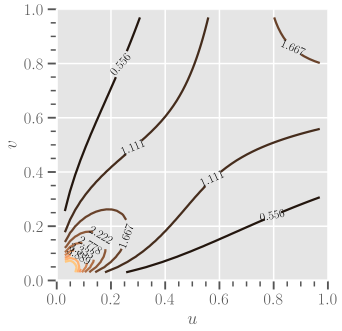
\includegraphics[width=.8\linewidth]{02_ClaytonCopula_contour}
		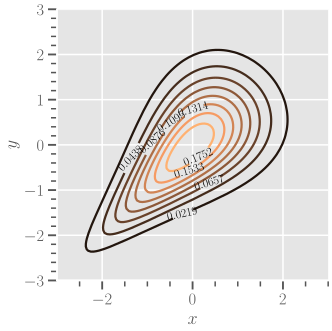
\includegraphics[width=.8\linewidth]{02_ClaytonCopula_contour_norm}
	\end{minipage}
	\caption{Gęstość kopuły Claytona, $\delta = 1.2$: powierzchnia (lewy panel), kontur w skali kopuły (prawy górny panel), kontur w skali brzegowo-znormalizowanej (prawy dolny panel). \label{fig:clayton_copula_density}}
\end{figure}

\begin{df}[Kopuła Gumbela]
	Kopuła Gumbela to kopuła archimedejska o generatorze $\phi(t;\delta) = (-\ln t)^{\delta}$. Jest ona jednoparametryczną kopuła, wyrażoną poprzez dystrybuantę zadaną wzorem:
	
	$$ C(u_1, u_2; \delta) = \exp\big[-[(-\ln u_1)^\delta+(-\ln u_2)^\delta]^{\frac{1}{\delta}}\big],$$
	dla $\delta \geqslant 1.$
\end{df}
\begin{prop}
	Dla kopuły Gumbela o parametrze $\delta$, współczynnik Kendalla wynosi:
	$$ \tau = \frac{\delta}{\delta + 2}.$$
	
	Współczynniki zależności ogonów wynoszą zaś odpowiednio:
	\begin{equation} \label{eq1}
		\begin{split}
			\lambda^{l}&=0\\
			\lambda^{u}&=2 - 2^{\frac{1}{\delta}}.
		\end{split}
	\end{equation}
\end{prop}
Kopuła Gumbela również pozwala modelować niesymetryczne zależności zmiennych losowych.  Rysunek \ref{fig:gumbel_copula_density} przedstawia powierzchnię gęstości i kontury w przypadku $\delta = 1.8$, gdzie widzimy powyższą niesymetryczność. Ta rodzina nie jest jednak wyczerpującą, ponieważ mamy jedynie $C(u,v;\delta = 1) = C^{\perp}$, oraz $C(u,v;\delta \to \infty) \to C^{+}$, natomiast kopuła $C^{-}$ nie jest częścią tej rodziny. \\
Kopuły Gumbela mogą więc posługiwać do modelowania jedynie dodatnich zależności, lub w granicznym przypadku niezależności. Nie przeszkodziło to jednak w skutecznej aplikacji tych kopuł do badań klinicznych, gdzie spopularyzował je Hougaard, w \cite{Hougaard1986} wykorzystując do testowania hipotez o pozytywnym wpływie leku przeciw guzom na długość życia szczurów w grupie leczenia.

\begin{figure}[h]
	\centering
	\begin{minipage}{0.5\linewidth}
		\includegraphics[width=\linewidth]{02_GumbelCopula_density}
	\end{minipage}
	\begin{minipage}{0.45\linewidth}
		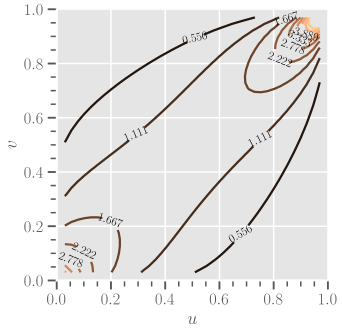
\includegraphics[width=.8\linewidth]{02_GumbelCopula_contour}
		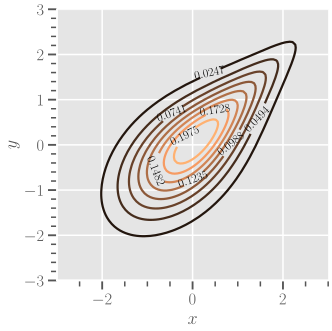
\includegraphics[width=.8\linewidth]{02_GumbelCopula_contour_norm}
	\end{minipage}
	\caption{Gęstość kopuły Gumbela, $\delta = 1.8$: powierzchnia (lewy panel), kontur w skali kopuły (prawy górny panel), kontur w skali brzegowo-znormalizowanej (prawy dolny panel). \label{fig:gumbel_copula_density}}
\end{figure}

\begin{df}[Kopuła Franka]
	Kopuła Franka to kopuła archimedejska o generatorze $\phi(t;\delta) = -\ln\frac{\exp(-\alpha t) - 1}{\exp(-\alpha)-1}$. Jest ona jednoparametryczną kopuła, wyrażoną poprzez dystrybuantę zadaną wzorem:
	
	$$ C(u_1, u_2; \delta) = -\frac{1}{\delta}\ln\big[ \frac{1}{1-e^{-\delta}}[(1-e^{-\delta}) - (1-e^{-\delta u_1})(1-e^{-\delta u_2})] \big],$$
	dla $\delta \in (-\infty; 0) \cup (0; \infty).$
\end{df}
\begin{prop}
	Dla kopuły Franka o parametrze $\delta$, współczynnik Kendalla wynosi:
	$$ \tau = 1 + 4[D(\delta) - 1]/\delta,$$
	gdzie $D(\alpha)$ to:
	$$ D(\alpha) = \frac{1}{\alpha} \int_{0}^{\alpha} \frac{t}{\exp(t) - 1}dt.$$
		
	Współczynniki zależności ogonów wynoszą zaś odpowiednio:
	\begin{equation} \label{eq1}
		\begin{split}
			\lambda^{l}&=0\\
			\lambda^{u}&=0.
		\end{split}
	\end{equation}
\end{prop}
Rodzina kopuł Franka jest rodziną wyczerpującą, bowiem $C(u,v;\delta = 0) = C^{\perp}$, $C(u,v;\delta \to \infty) \to C^{+}$, oraz $C(u,v;\delta \to -\infty) \to C^{-}$ . Kopuła Franka jako jedyna z wymienionych kopuł archimedejskich jest symetryczna. Rysunek \ref{fig:frank_copula_density} przedstawia powierzchnię gęstości i kontury w przypadku $\delta = 5$. \\
Jedno z ciekawych jej zastosowań, przedstawia \cite{Jianwei2021}. W swojej pracy Jianwei rozważa problem optymalizacji częstości ładowania pojazdów elektrycznych. Kopuła Franka jest przez niego używana do modelowania zależności między siłą wiatru, a ilością energii z ogniw fotowoltaicznych, co wykorzystuje do wyznaczenia optymalnej strategii ładowania pojazdu, która stabilizuje popyt/podaż na energię w sieci energetycznej, skutkując w niższych kosztach utrzymania pojazdu. 

\begin{figure}[h]
	\centering
	\begin{minipage}{0.5\linewidth}
		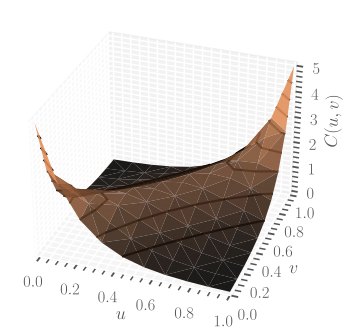
\includegraphics[width=\linewidth]{02_FrankCopula_density}
	\end{minipage}
	\begin{minipage}{0.45\linewidth}
		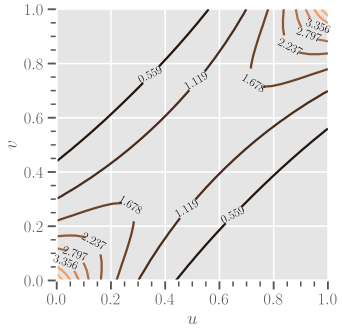
\includegraphics[width=.8\linewidth]{02_FrankCopula_contour}
		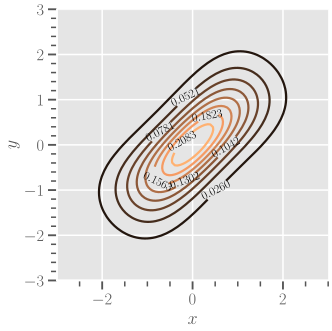
\includegraphics[width=.8\linewidth]{02_FrankCopula_contour_norm}
	\end{minipage}
	\caption{Gęstość kopuły Franka: powierzchnia (lewy panel), kontur w skali kopuły (prawy górny panel), kontur w skali brzegowo-znormalizowanej (prawy dolny panel). \label{fig:frank_copula_density}}
\end{figure}

\underline{Rodzina kopuł \emph{extreme-value}}
\vspace{0.5cm}

Ostatnią z prezentowanych metod konstrukcji kopuł jest konstrukcja asymptotyczna, poprzez teorię wartości ekstremalnych.\\
Zakładając, że $X_1$ i $X_2$ są dwoma zmiennymi losowymi o rozkładach $F_1$, $F_2$, zdefiniujemy kopułę \emph{extreme-value} jako kopułę odpowiadającą za zależność pomiędzy maksimum z $n$ realizacji $X_1$ a maksimum z $n$ realizacji $X_2$. 

\begin{df}[Kopuła \emph{extreme-value}]
	Dwuwymiarowa kopuła $C$ nazywana jest kopułą \emph{extreme-value}, jeżeli istnieje dwuwymiarowa kopuła $C_X$, taka że dla $n\to\infty$ mamy:
	
	$$ [C_X(u_1^{\frac{1}{n}}, u_2^{\frac{1}{n}})]^n \to C(u_1, u_2) \forall_{(u_1, u_2)}\in [0,1]^2.$$
	
	Mówimy wówczas, że kopuła $C_X$ jest w obszarze przyciągania kopuły $C$.
\end{df}

To samo można zdefiniować posługując się pojęciem kopuł \emph{max-stabilnych}
\begin{df}[Kopuła max-stabilna]
	Dwuwymiarowa kopuła $C$ nazywana jest kopułą max-stabilną, jeśli spełnia warunek:
	
	$$ C(u_1, u_2) = [C(u_1^{\frac{1}{n}}, u_2^{\frac{1}{n}})]^n,$$
	Dla każdej liczby całkowitej $n\geqslant 1$, oraz dla każdej pary ${(u_1, u_2)}\in [0,1]^2.$
	
\end{df}
\begin{thm}
	Dwuwymiarowa kopuła $C$ jest kopułą \emph{extreme-value}, tylko i tylko wtedy gdy jest max-stabilna.
\end{thm}

Przykładem kopuły \emph{extreme-value} z podanych już wcześniej jest kopuła Gumbela. Inną, nietypową, ale często spotykaną kopułą z tej rodziny jest kopuła Marshalla-Olkina.

\begin{df}[Kopuła Marshalla-Olkina]
	Dwuwymiarową kopułą Marshalla-Olkina o parametrach $m$ i $n$ nazwiemy kopułę o dystrybuancie:
	
	$$ C(u_1, u_2; m,n) = \min[u_1^{1-m}u_2; u_1u_2^{1-n}].$$
	Gęstość tej kopuły zadana jest przez:
	
	$$
	c(u_1, u_2;m,n)=
	\begin{cases}
		(1-m)u_1^{-m},\text{ dla }u_1^m>u_2^n\\
		(1-n)u_2^{-n},\text{ dla }u_1^m<u_2^n
	\end{cases}
	$$	
\end{df}
\begin{prop}
	Dla kopuły Marshalla-Olkina o parametrach $m,n$, współczynnik Kendalla wynosi:
	$$ \tau = \frac{mn}{m-mn+n}.$$
	
	Współczynniki zależności ogonów wynoszą zaś odpowiednio:
	\begin{equation} \label{eq1}
		\begin{split}
			\lambda^{l}&=0\\
			\lambda^{u}&=min(m,n).
		\end{split}
	\end{equation}
\end{prop}
Kopuła Marshalla-Olkina jest nietypowa, bo posiada część ciągłą, o powyższej gęstości, jak i część singularną wzdłuz krzywej $u_1^m=u_2^n$. Ta rodzina nie jest wyczerpująca, ponieważ nie zawiera $C^{-}$. Natomiast dla $m=0 \vee n=0$ mamy $C^{\perp}$, a przy $m=1=n$ dostajemy $C^{+}$. \\
Kopuły Marshalla-Olkina powstają naturalnie w teorii niezawodności systemów. Rozważając system o wielu komponentach, gdzie awaria dowolnego komponentu powoduje awarię całego systemu, w klasycznym podejściu zakłada się rozkład wykładniczy dla czasu życia każdego z komponentów (z powodu braku pamięci), oraz niezależność między komponentami. W praktyce jednak, czasy do awarii poszczególnych komponentów nie są niezależne: do modelowania tej zależności dużo lepiej służy właśnie kopuła Marshalla-Olkina \cite{Matus2019}.\\

\begin{figure}[h]
	\centering
	\begin{minipage}{0.5\linewidth}
		\includegraphics[width=\linewidth]{02_MarshallOlkinCopula_density}
	\end{minipage}
	\begin{minipage}{0.45\linewidth}
		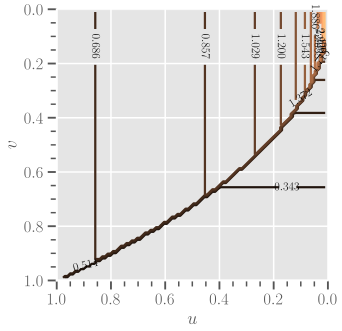
\includegraphics[width=.8\linewidth]{02_MarshallOlkinCopula_contour}
		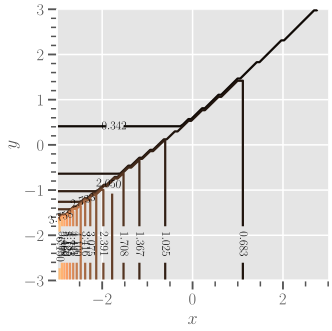
\includegraphics[width=.8\linewidth]{02_MarshallOlkinCopula_contour_norm}
	\end{minipage}
	\caption{Gęstość kopuły Marshalla-Olkina, $m=0.35,n=0.75$: powierzchnia (lewy panel), kontur w skali kopuły (prawy górny panel), kontur w skali brzegowo-znormalizowanej (prawy dolny panel). \label{fig:marshall_olkin_copula_density}}
\end{figure}




\label{subsec:dwuwymiarowe_kopuly_przyklady}



\section{Pair Copula Constructions}
\label{sec:pair_copula_constructions}
\subsection{Wielowymiarowe kopuły}
\label{subsec:wielowymiarowe_kopuly}
		
\subsection{Pair Copula Constructions}
\label{subsec:pair_copula_constructions}
	
\subsection{Vine Copula}
\label{subsec:vine_copula}


\section{Vine Copulas}
\label{sec:vine_copulas}
Problemy z którymi spotykamy się w praktyce są nierzadko z natury wielowymiarowe. W rozdziale \ref{sec:popularne_spready} opowiemy o clean dark spreadach, czyli mierze rentowności elektrowni węglowej który wymaga modelowania zależności trzech komponentów (ceny węgla, ceny certyfikatów emisyjnych i ceny prądu). Model LDA dla ryzyka operacyjnego nadmieniony w rozdziale \ref{subsec:dwuwymiarowe_kopuly_przyklady} wymaga segmentacji strat względem przynależności do jednej z kilkunastu/kilkudziesięciu homogenicznych kategorii (ORC) i modelowania zależności między nimi. Natomiast modelowanie zależności komponentów portfela inwestycyjnego może okazać się problemem o wymiarowości rzędu setek.\\
Widzimy więc, że przekrój zastosowań praktycznych jest bardzo duży i istnieje zapotrzebowanie na wielowymiarowe modele zależności. Dwuwymiarowe kopuły przedstawione w \ref{subsec:dwuwymiarowe_kopuly_przyklady} mają często swoje wielowymiarowe odpowiedniki (\cite{Cherubini_Copula_Methods_in_Finance}, \cite{Kurowicka_Dependence_Modeling}). Są one jednak stosunkowo mało elastyczne, ponieważ nie pozwalają "dostroić" modelu na poziomie interakcji każdej pary wymiarów zmiennej losowej. W tym rozdziale sięgniemy po modele Vine Copula, które pozwolą bardzo granularnie modelować wielowymiarowe zależności, do stopnia gdzie będziemy w stanie określić zależność między dowolnymi dwoma rozkładami brzegowymi.\\

\subsection{Pair Copula Constructions}
\label{subsec:pair_copula_constructions}
\subsection{Wielowymiarowe kopuły}
\label{subsec:wielowymiarowe_kopuly}
		
\subsection{Pair Copula Constructions}
\label{subsec:pair_copula_constructions}
	
\subsection{Vine Copula}
\label{subsec:vine_copula}

	
\subsection{Vine Copula}
\label{subsec:vine_copula}
Ideę rozbijania rozkładu na dwuwymiarowe bloki da się rozszerzyć na $d$-wymiarów. Podobnie jednak jak w przykładzie 3-wymiarowym z sekcji \ref{subsub:przyklad_3_wymiary}, nie mamy jedyności tej reprezentacji - istnieje wiele różnych dróg do osiągnięcia tego samego celu. 

\begin{thm}[$d$-wymiarowa PCC]
	Niech $f_{1,2,\dots,d}$ będzie gęstością łączną $d$-wymiarowego rozkładu. Możemy ją wyrazić poprzez:
	
	\begin{equation}
		f_{1,\dots, d}(x_1, \dots, x_d) = \bigg[ \prod_{j=1}^{d-1} \prod_{i=1}^{d-j} c_{i, (i+j); (i+1)\dots(i+j-1)} \bigg] \cdot \bigg[ \prod_{k=1}^{d}f_k(x_k)\bigg].
	\end{equation}
\end{thm}
\begin{proof}
	Zacznijmy od rozważenia rozkładu łącznego i jego ogólnej dekompozycji:
\begin{equation}
	\begin{split}
		f_{1, \dots, d}(x_1, \dots, x_d) &= f_{d|1 , \dots, d-1}(x_d|x_1, \dots, x_{d-1})f_{1,\dots,d-1}(x_1, \dots, x_{d-1})\\
		&=\dots= \bigg[\prod_{t=2}^{d}f_{t|1,\dots,t-1}(x_t|x_1, \dots, x_{t-1})\bigg]\cdot f_1(x_1)
	\end{split}
	\label{eq:d-dimensional_decomp}
\end{equation}

Teraz użyjemy lematu \ref{lem:copula_representation_of_conditional_density} do rozkładu warunkowego $(X_1, X_t) | (X_2, \dots, X_{t-1})$ żeby rekursywnie wyrazić $f_{t|1,\dots,t-1}(x_t|x_1,\dots,x_{t-1})$.
	\begin{equation}
	\begin{split}
	f_{t|1,\dots,t-1}(x_t|x_1,\dots,x_{t-1})&= c_{1,t|2,\dots,t-1}\cdot f_{t|2,\dots,t-1}(x_t|x_2,\dots,x_{t-1})  \\
	& = \bigg[ \prod_{s=1}^{t-2} c_{s,t;s+1,\dots,t-1} \bigg] c_{(t-1), t} f_t(x_t).	
	\end{split}
	\label{eq:recursive_pcc}
	\end{equation}

Aplikując \ref{eq:recursive_pcc} do równania \ref{eq:d-dimensional_decomp}, oraz oznaczając $s=i, t=i+j$ możemy zapisać:

\begin{equation*}
	\begin{split}
		f_{1, \dots, d}(x_1, \dots, x_d) &= \bigg[\prod_{t=2}^{d}\prod_{s=1}^{t-2} c_{s,t;s+1,\dots,t-1}\bigg] \cdot \bigg[ \prod_{t=2}^{d}c_{(t-1), t} \bigg] \cdot \bigg[ \prod_{k=1}^{d}f_{k}(x_k) \bigg] = \\
		& = \bigg[\prod_{j=1}^{d-1}\prod_{i=1}^{d-j}c_{i,(i+j);(i+1)\dots(i+j-1)}\ \bigg] \cdot \bigg[\prod_{k=1}^{d}f_k(x_k)\bigg].
	\end{split}
\end{equation*}
\end{proof}

Jak widać z równania \ref{eq:d-dimensional_decomp}, dekompozycje te potrafią być zawiłe i mało interpretowalne. Dlatego poniżej wprowadzimy fragmenty teorii grafów, która pozwoli nam lepiej komunikować te dekompozycje.


\section{Przykłady zastosowań modeli kopułowych}
\label{sec:przyklady_zastosowan_modeli_kopulowych}
		
\mgrclosechapter
\chapter{Spready na rynkach finansowych}

\section{Popularne rodzaje spreadów}
\section{Modelowanie spreadów}
\section{Model kopułowy}


\mgrclosechapter
\begin{wstep}[Wnioski]    % ew. \begin{wstep}[Wprowadzenie]
	W pracy omówiliśmy model ARIMA-GARCH-VineCopula w kontekście symulacji spreadu wielu aktywów. Podaliśmy teorię kopuł, oraz struktur Vine Copula z wyszczególnieniem ich zastosowań w praktyce, oraz omówiliśmy ich związek z rodzajami struktur zależności alternatywnymi dla najprostszej liniowej korelację Pearsona.\\
	Przedstawiliśmy wyniki kalibracji modelu do tygodniowych cen zamknięcia komponentów \emph{soybean crush spreadu}. W trakcie analizy udowodniliśmy ciężkoogonowość logzwrotów, oraz brak istotnej struktury autokorelacji czy częściowej autokorelacji w komponentach spreadu. Dane przejawiają heteroskedastyczność, dającą się skutecznie zamodelować przy pomocy modelu GARCH(2, 3).\\
	Zbadana została struktura zależności reziduów modeli GARCH, do których dopasowany został model Vine Copula bazujący na kopułach: Gaussowskiej i Franka. Model ukazał istotność soi jako wiodącego szeregu czasowego o największym wpływie na pozostałe komponenty, oraz wskazał na brak istotnej zależności w ogonach reziduów co przejawiło się w dopasowaniu kopuł o braku współczynnika zależności ogonów.\\
	Porównaliśmy model Vine Copula z modelem wielowymiarowej kopuły gaussowskiej dochodząc do wniosku, że oba modele uchwycają ciężkoogonowość spreadu, oraz dają podobne rozkłady logzwrotów dla większości kwantyli - jednak Vine Copula przejawia cięższe ogony w kwantylach ekstremalnych ($0.01$, $0.99$).\\
	Finalny symulacyjny model potrafi produkować realistyczne realizacje trajektorii spreadu, co pozwala wykorzystywać go do wyceny instrumentów pochodnych na spread metodą Monte Carlo - co zaprezentowane zostało dla przypadku europejskich opcji.
	
\end{wstep}


% \appendix
% \chapter{----}
%%
%-> Treść dodatku A
%%
% \mgrclosechapter
%%
%%
%\bibliographystyle{bibliography_style}
\bibliography{bibliography.bib} 
\end{document}

%% =========================================================== %%